\subsection*{Standard floating figures.}
Figure \ref{fig:PumpDrawing} is wrapped into a standard floating environment. That means that \LaTeX will determine the exact placement of the figure. Even though you can state preferences (see code) it can be tricky to get the right placement - especially when working on very tight manuscripts. If you want exact placement, add \verb!\usepackage{float}! to this file's header and use [H] in the figure environment's placement options.

Figure of the protocol \ref{fig:PumpDrawing}

\begin{figure*}
	\centering
	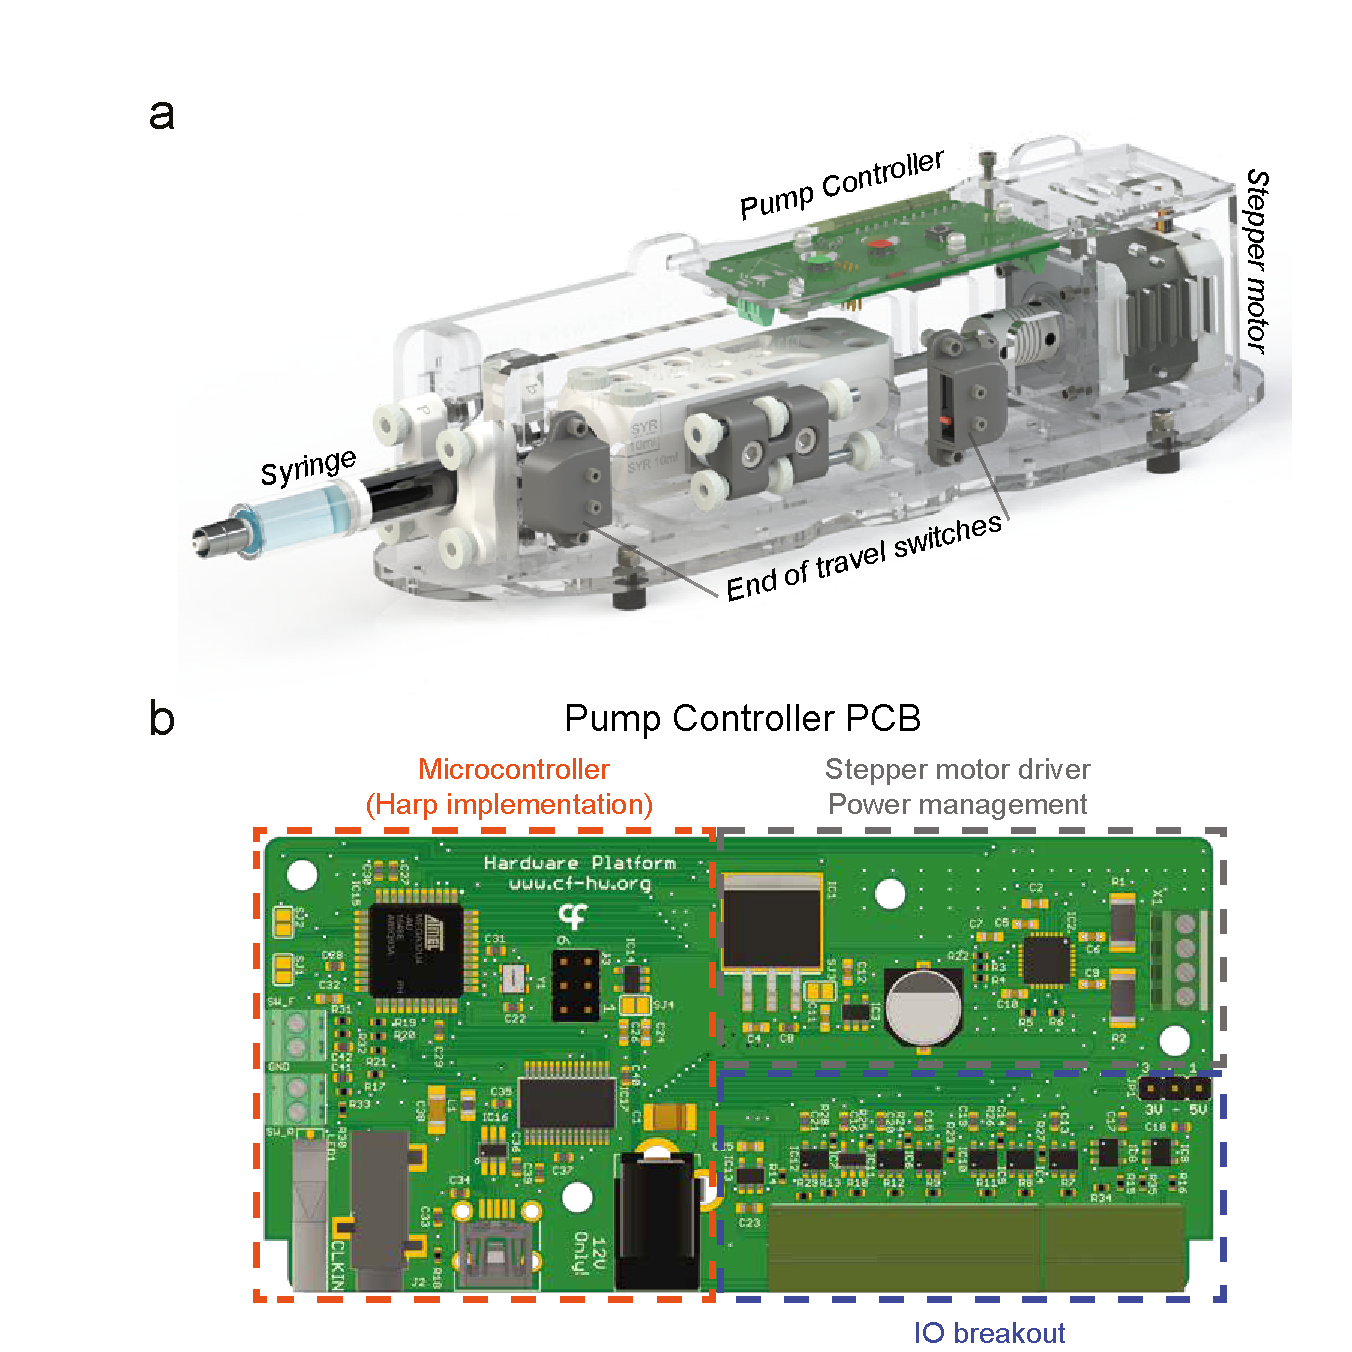
\includegraphics[width=1.0\linewidth]{Figures/Artboard 1.pdf}
	\caption{\textbf{Syringe pump system.}\\
		(\textbf{A}) 3D model of the fully assembled syringe pump system. Controller PCB, Syringe, switches, and stepper motor are highlighted.  \textbf{B}) Diagram of Controller PCB. The three main sections of the board are highlighted: Microcontroller, which implements the Harp protocol; Motor driver and power management, which provide the low-level logic to drive the stepper motor, and the I/O breakout, that affords users with input and output lines which can be used to control and monitor the function of the system, respectively. See \TODO{miss ref} \hyperref[s:methods]{Methods} for further details}
	\label{fig:PumpDrawing}
\end{figure*}



Another figure \ref{fig:PumpProtocol}
\begin{figure} 
	\centering
	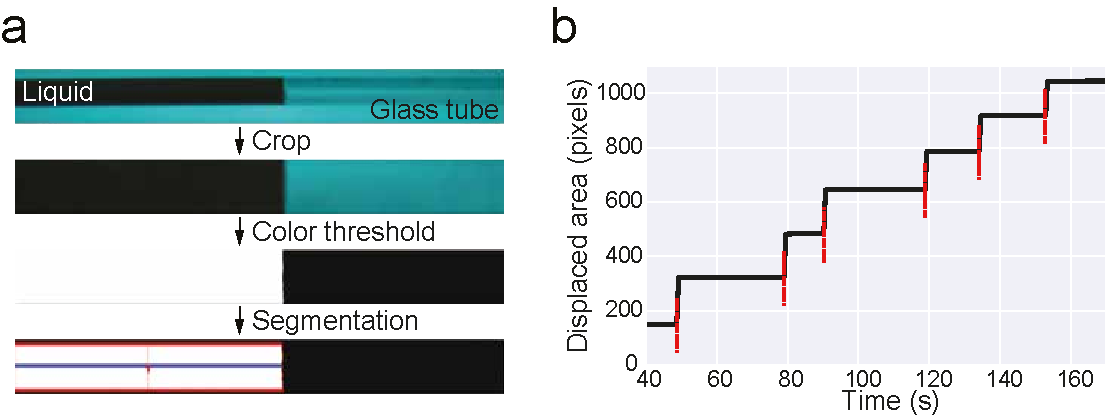
\includegraphics[width=1.0\linewidth]{Figures/Artboard 1_1.pdf}
	\caption{\textbf{Tracking small single-bolus events.}\\
		 (\textbf{A}) Schematic of th computer vision algorithm followed to measure small, microliter range, volumes. Briefly, from top to bottom, we cropped, thresholded and segmented the area of the capillary filled with liquid. We took its area  as a proxy of delivered volume. (\TODO{ref missing}See Methods for further details)  \textbf{B}) Example trace of the measured area in A), as a function of time during one of the experiments. Red vertical dashed lines represent liquid delivery events (calibrated to \TODO{x uL}).}
	\label{fig:PumpProtocol} 
\end{figure}

Another figure \ref{fig:PumpControl}
\begin{figure}
	\centering
	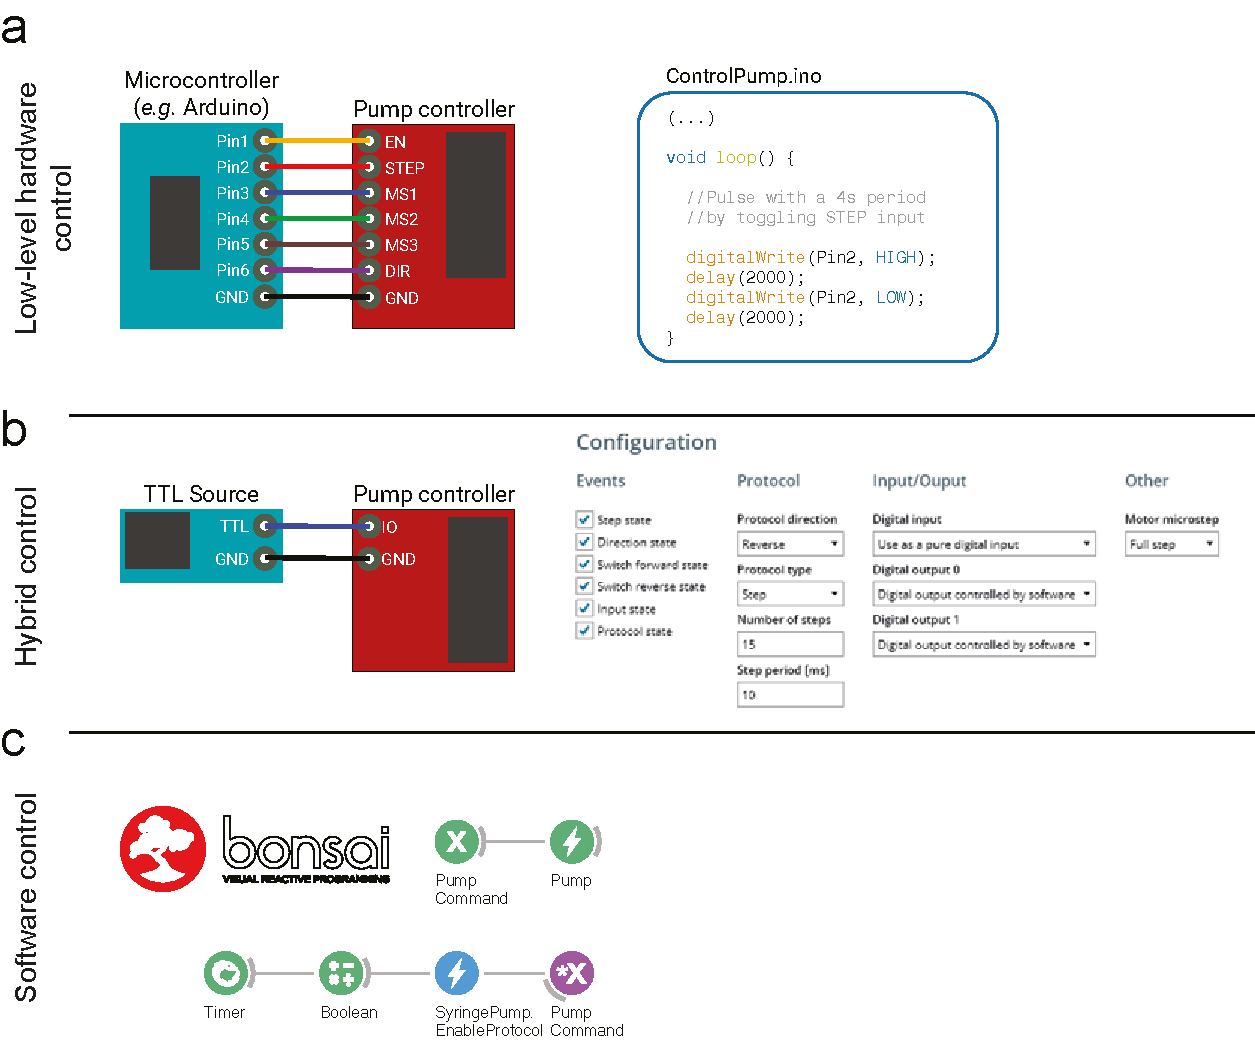
\includegraphics[width=1.0\linewidth]{Figures/Artboard 4.pdf}
	\caption{\textbf{The current system affords three distinct levels of control.}\\
		(\textbf{A}) blah }

	\label{fig:PumpControl} 
\end{figure}



Mention:
 that identical y axis were used for the calibration;
 probably a non-linear region could be achieved if we kept dropping the valve opening time
 
Another figure \ref{fig:PumpVsValve}
\begin{figure} 
	\centering
	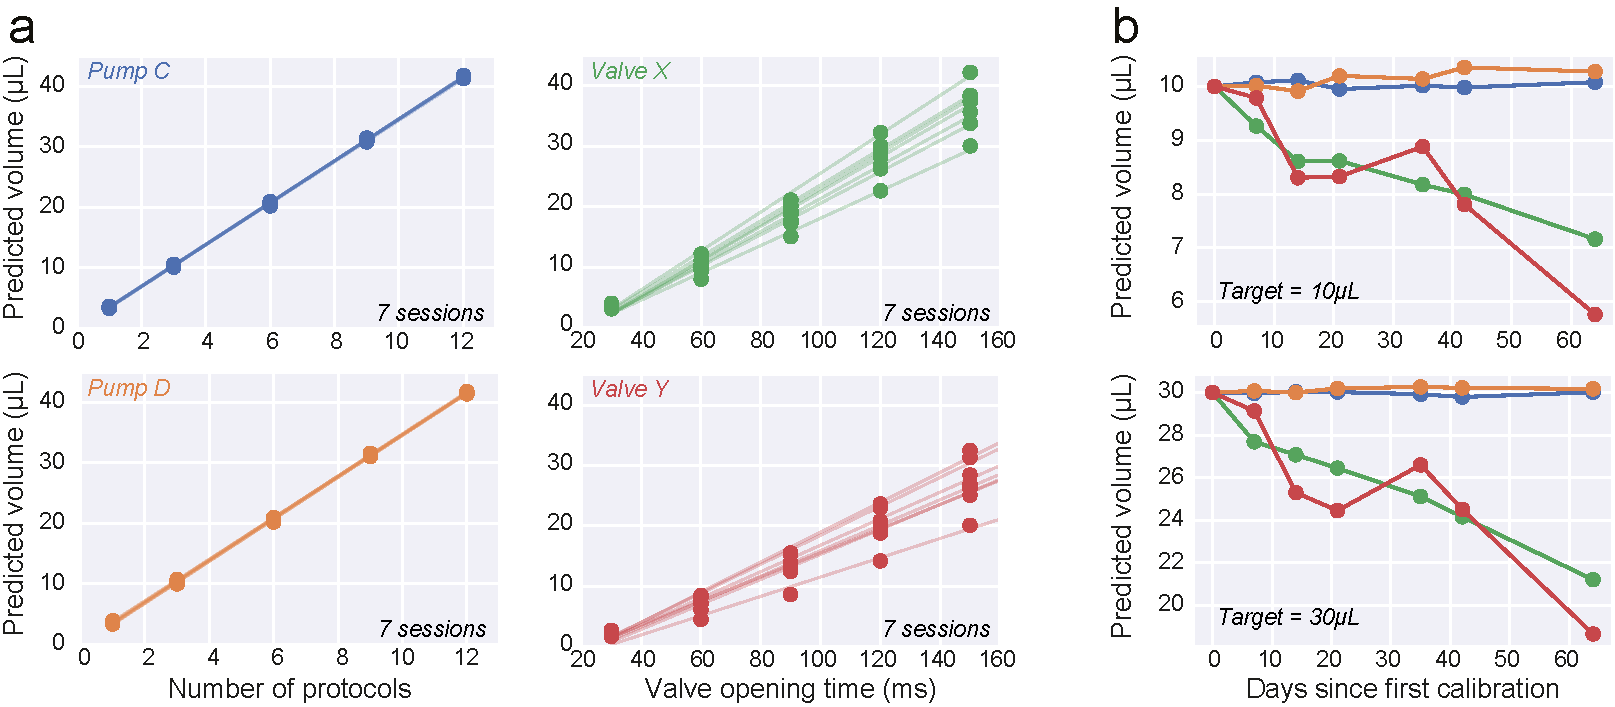
\includegraphics[width=1.0\linewidth]{Figures/Artboard 2.pdf}
	\caption{\textbf{Comparison of calibration stability between the a gravity-based solution and the presented pump system.}\\
		(\textbf{A}) For each system we followed a calibration protocol (\TODO{see methods}) wherein we measured the amount of delivered liquid as a function of number of pre-programmed delivery protocols or valve opening time, for the \textit{Pump} (left) and \textit{Valve} (right) solutions, respectively. Where volumes in similar ranges were probed. Individual shown fits correspond to single calibration protocols. For each system we tested two devices independently.  (\textbf{B}) Predicted delivery volume for two arbitrary volumes (10 and 30 \TODO{microlitters}, top and bottom, respectively) based on the calibration linear fits derived from A). For each day, we used the calculated fit to estimate how much volume would have been delivered had we kept the values from Day 0}
	\label{fig:PumpVsValve} 
\end{figure}


Non linear, so probably needs to be calibrated. Likely not only a function of the IPI but also the flow path resistance
Another figure \ref{fig:FlowRateControl}
\begin{figure}
	\centering
	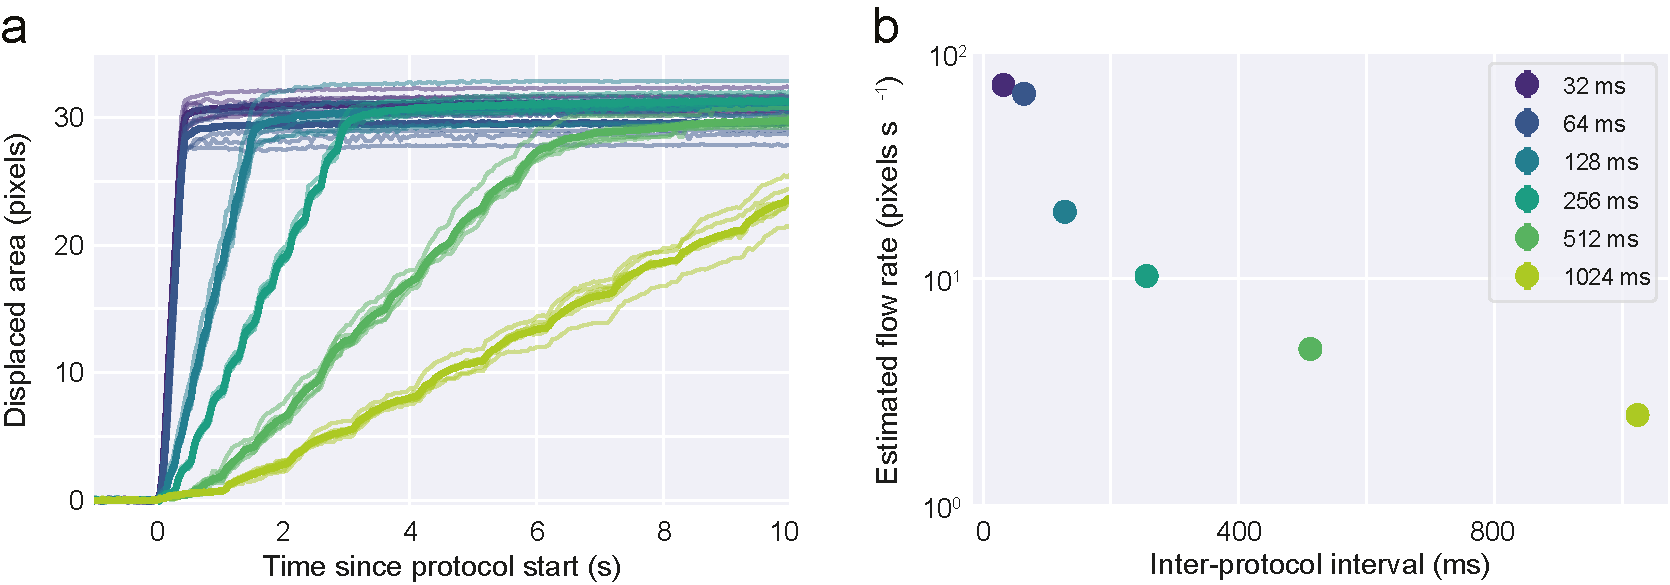
\includegraphics[width=1.0\linewidth]{Figures/Artboard 3.pdf}
	\caption{\textbf{Syringe pump affords dynamic control over flow rate.}\\
		  (\textbf{A}) Time course of delivered volume (displaced pixel area, see methods for details) aligned on protocol onset (t = 0) for different (distinct colors) Inter-protocol-interval values (IPI). Thin and thick lines represent single trials and averages for a given IPI, respectively. (\textbf{B}). Estimated flow rate (pixels s$^{-1}$) for all tested IPI (mean $\pm$ std., n = 6 for each IPI). All data was obtained form a single device.}
	\label{fig:FlowRateControl} 
\end{figure}

Another figure \ref{fig:SingleStepCalibration}
\begin{figure}
	\centering
	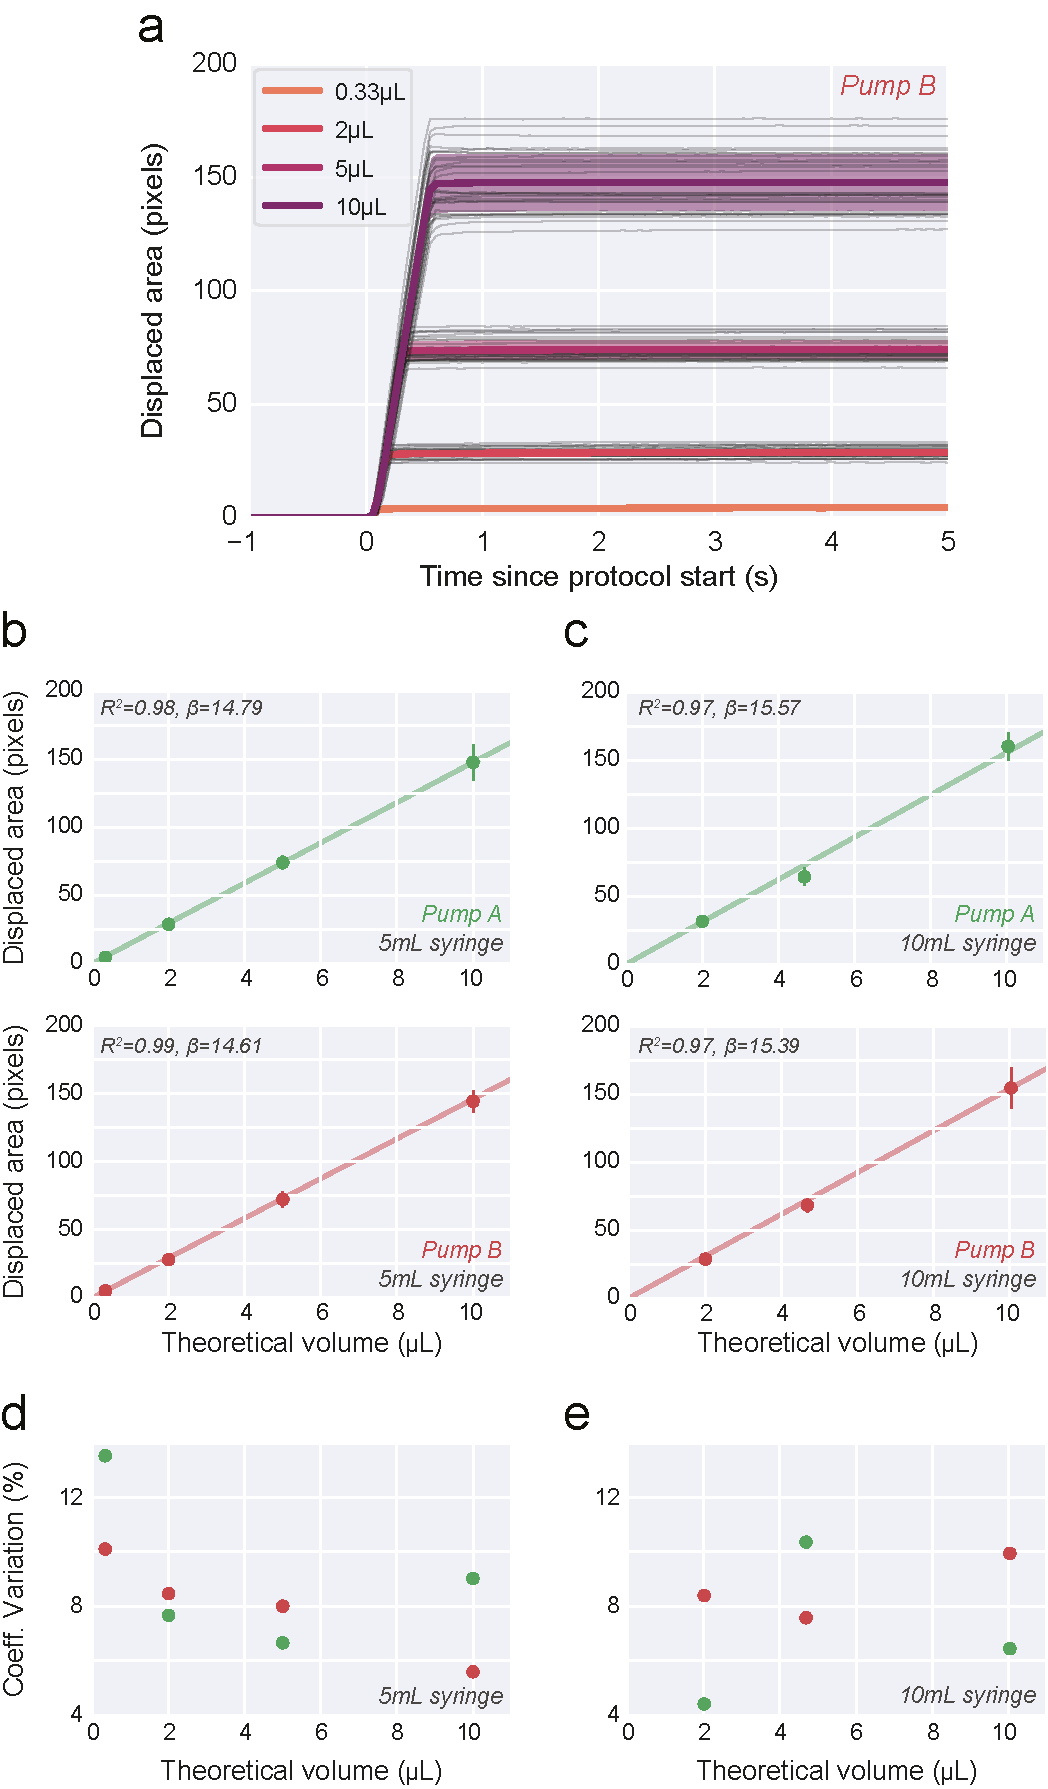
\includegraphics[width=1.0\linewidth]{Figures/Artboard 5.pdf}
	\caption{\textbf{Single-bolus protocol calibration}.\\
		 (\textbf{A}) Time course of delivered volume aligned on protocol onset (t = 0) for different theoretically expected delivered volumes (distinct colors). Thin and thick lines correspond to single trials and averages for a given expected volume, respectively. \textbf{B, C}) Displaced area for the different delivered liquid amounts. Each point shows mean $\pm$ std. across 30 replicates, per volume, in two different pumps (\textit{PumpA} and \textit{PumpB}, green and red, respectively) and using two different syringe models (5 and 10 mL, \textbf{B} and \textbf{C}, respectively). \textbf{D, E}) Coefficient of variation ($\sigma / \mu$) calculated from the data shown in \textbf{B} and \textbf{C}, respectively.}
	\label{fig:SingleStepCalibration} 
\end{figure}


Another figure \ref{fig:LargeVolumeCalibration}
\begin{figure}[ht] 
	\centering
	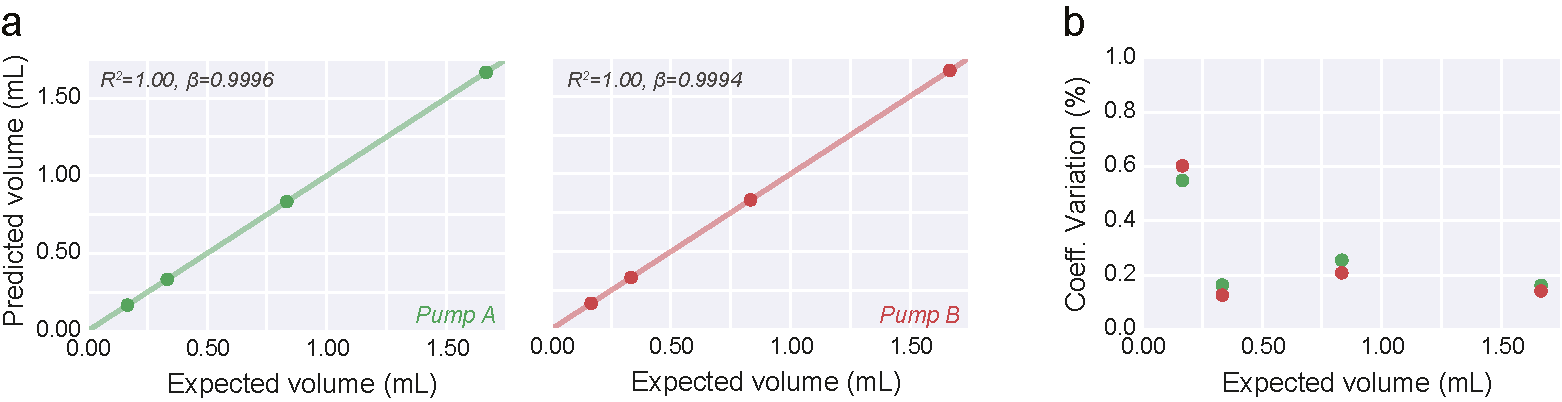
\includegraphics[width=1.0\linewidth]{Figures/Artboard 6.pdf}
	\caption{\textbf{Large volume protocol calibration}.\\
	(\textbf{A}) Delivered volume (mean $\pm$ std.) across 20 performed delivery protocols for four distinct large volume amounts, in two pump systems (\textit{PumpA} and \textit{PumpB}, green and red, respectively). \textbf{B}) Coefficient of variation ($\sigma / \mu$) calculated from the data shown in \textbf{A}.}

	\label{fig:LargeVolumeCalibration} 
\end{figure}


Sofia s figure \ref{fig:Behavior}
\begin{figure}[ht] 
	\centering
	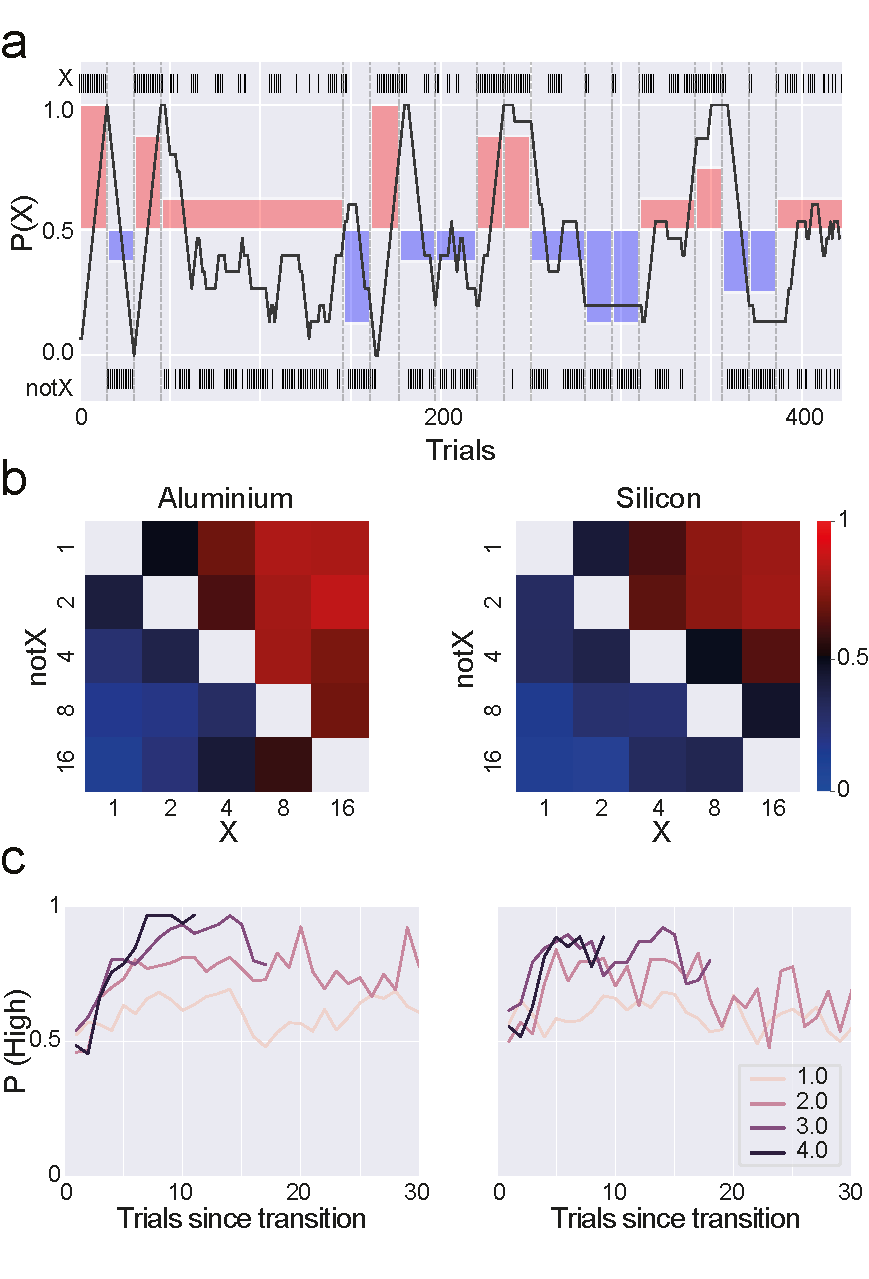
\includegraphics[width=1.0\linewidth]{Figures/Artboard 9.pdf}
	\caption{\textbf{Rat's behavior}.\\
		(\textbf{A}) Probability of choosing reward giving nose-port X as a function of the possible reward amount combinations given by each nose-port. Values in the heatmap axes are the number of protocols given on each reward delivery, by each reward nose-port (X and notX). (\textbf{B}) Probability of choosing the highest rewarded side over the trials following block transition. Lines correspond to the absolute value of the difference between rewards at each nose-port in logarithmic units (base 2). The highest the difference between the two rewards available on a particular block, the sooner animals converge to the highest rewarded nose-port, [suggesting the need for fewer reward samples (trials) as the difference between rewards increases]. }
	
	\label{fig:Behavior} 
\end{figure}

ephys s figure \ref{fig:Ephys}
\begin{figure}[ht] 
	\centering
	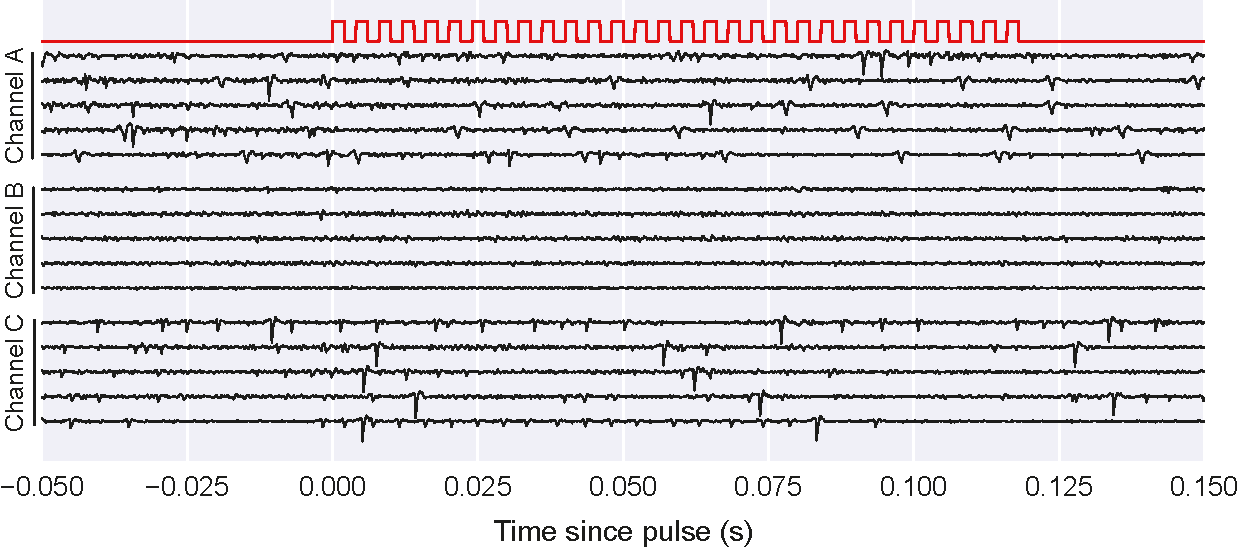
\includegraphics[width=1.0\linewidth]{Figures/Artboard 7.pdf}
	\caption{\textbf{Single-bolus protocol calibration}.\\
	(\textbf{A}) blahblah }	
	\label{fig:Ephys}
\end{figure}



%\SI{10}{\micro\meter}
